\documentclass{article}

% Imports
\usepackage[a4paper, total={6in, 8in}]{geometry} % Imposta i margini della pagina
\usepackage{array} % Fornisce per le tabelle il tipo di colonna "m", che consente di impostare una larghezza fissa
\usepackage{tabularray} % Fornisce per le tabelle i tipi di colonna che permettono l'allineamento verticale
\usepackage{booktabs} % Fornisce decoratori per le tabelle
\usepackage{graphicx} % Inserimento immagini

% Use case descriptions imports & settings
\usepackage[dvipsnames, table]{xcolor} % Per colorare celle delle tabelle
\usepackage{tabularx}
\usepackage{enumitem}
\setlist[enumerate]{label*=\arabic*., topsep=0pt, itemsep=0pt, parsep=0pt, partopsep=0pt} % Imposta gli indici di tutti i livelli di enumerazione come numeri arabi (invece del default che passa alle lettere) e rimuove il padding
\usepackage{float} % Fornisce la posizione 'H' per le tabelle, che le posiziona direttamente dove specificato nel codice latex e non in cima alla pagina o altri comportamenti 'float' non desiderati

% Macros
\newcommand{\mycount}[1]{\stepcounter{#1}\arabic{#1}}

\title{Tell: Gestore teatrale}
\date{2025-06-20}
\author
{
    Giuseppe Mariotti \\
    Riccardo Ripa \\
    Rodrigo Rengifo \\
    Mattia Praolini
}

\begin{document}
    \pagenumbering{gobble}
    \maketitle
    \newpage
    \pagenumbering{arabic}

    \section{Panoramica}
        Il progetto prevede la realizzazione di un applicativo che consenta la vendita di biglietti per eventi teatrali (come opere e concerti) e la divulgazione di informazioni a riguardo. Il sistema si articolerà, per l’acquirente, in due sezioni: la prima conterrà la lista di eventi disponibili all'acquisto, la seconda conterrà maggiori informazioni riguardo le opere, incluse quelle non in programma al momento. Per la biglietteria saranno disponibili sezioni per la gestione degli eventi e delle prenotazioni, mentre per l'amministratore saranno disponibili sezioni per la gestione delle informazioni riguardo le opere e della struttura posti del teatro. Dall’intervista con i responsabili marketing e ufficio stampa di un ente pesarese operante nel settore sono emerse varie necessità. L’interfaccia dovrà essere ottimizzata per favorire la semplicità del processo di acquisto del biglietto: un’eccessiva quantità di informazioni in primo accesso ridurrebbe l’intuitività e l’accessibilità. Il prezzo di un biglietto è determinato dalla tipologia di posto scelto e dal tipo di evento, nonché da una lista di sconti applicabili in base a determinati criteri. Una volta confermata la prenotazione, il totem digitale stamperà una ricevuta contenente l'identificativo che potrà essere usato per effettuare il pagamento in biglietteria. Le voci delle informazioni dell’evento (direttore d’orchestra, interpreti, tecnici e altri) dovranno essere totalmente flessibili viste le notevoli differenze fra i vari tipi di eventi. Un caso particolare di eventi sono le opere, che possono essere messe in scena solo tramite una regia (una direzione artistica che accoppia alle musiche e al libretto dell’opera i costumi, fondali e altri elementi necessari alla rappresentazione). Infine, nella sezione anagrafica, per ogni opera dovrà essere memorizzato e mostrato all’utente lo storico delle regie presenti e passate.
    \newpage

    \section{Glossario dei termini}
        \begin{tblr}{h{3cm}h{2cm}m{10cm}}
            \hline
            \textbf{Termine} & \textbf{Sinonimi} & \textbf{Definizione} \\
            \hline
            Opera & N/A & Il testo e le musiche di un'opera lirica. Questi, a meno di casi li- mite che non interessano la realizzazione del software in questione, non vengono mai modificati. \\
            Regia & N/A & I costumi, i fondali, la direzione coreografica e degli effetti speciali e, in generale, della narrazione visiva dell'opera. Periodicamente le opere ricevono una nuova regia, che viene realizzata da un regista. \\
            Spettacolo & N/A & Le informazioni organizzative riguardo una determinata rappresentazione teatrale (di una \textbf{Regia} o altro tipo di spettacolo), come il cast, il direttore o il coro. \\
            Evento & N/A & La data e l'ora in cui un determinato spettacolo viene messo in scena. Solitamente, ciascuno spettacolo viene ripetuto in molteplici eventi. \\
            Cliente & N/A & L'aquirente di biglietti \\
            Biglietteria & N/A & Il dipendente dell'ufficio biglietteria \\
            Amministratore & N/A & Il gestore del sistema \\
            Utente & N/A & Uno qualunque tra \textbf{Cliente}, \textbf{Biglietteria} e \textbf{Amministratore} \\
            \hline
        \end{tblr}
    \newpage

    \section{Requisiti progettuali}
        \subsection{Diagramma}
            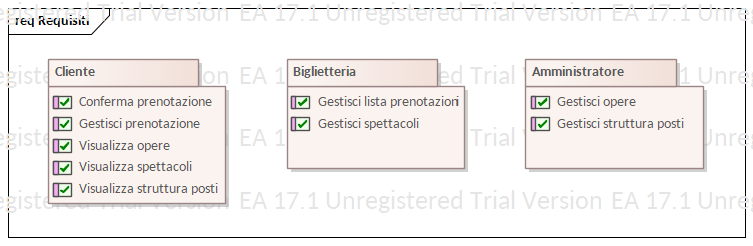
\includegraphics{imgs/requisiti/requisiti}

        \subsection{Requisiti Funzionali}
            \newcounter{rf}

            \subsubsection{Area Cliente}
                \textbf{RF\mycount{rf}: Visualizza opere} \\
                Il sistema dovrà mostrare al cliente le anagrafiche delle opere e l'archivio delle relative regie. \\
                \\
                \textbf{RF\mycount{rf}: Visualizza spettacoli} \\
                Il sistema dovrà mostrare al cliente la lista degli spettacoli e dei relativi eventi disponibili all'acquisto. \\
                \\
                \textbf{RF\mycount{rf}: Visualizza struttura posti} \\
                Il sistema dovrà consentire al cliente di visualizzare la struttura posti del teatro durante la composizione della prenotazione. \\
                \\
                \textbf{RF\mycount{rf}: Gestisci prenotazione} \\
                Il sistema dovrà consentire al cliente di creare una prenotazione e modificarne i posti o eliminarla completamente prima di averla confermata. \\
                \\
                \textbf{RF\mycount{rf}: Conferma prenotazione} \\
                Il sistema dovrà consentire al cliente di confermare la prenotazione, e produrre la ricevuta contenente l'identificativo della prenotazione per il pagamento alla cassa. \\

            \subsubsection{Area Biglietteria}
                \textbf{RF\mycount{rf}: Gestisci spettacoli} \\
                Il sistema dovrà consentire alla biglietteria di creare, modificare e rimuovere gli spettacoli in programma e i relativie eventi. \\
                \\
                \textbf{RF\mycount{rf}: Gestisci lista prenotazioni} \\
                Il sistema dovrà consentire alla biglietteria di visualizzare e modificare tutte le prenotazioni effettuate nel teatro e di contrassegnare le prenotazioni che sono state pagate in cassa. \\

            \subsubsection{Area Amministratore}
                \textbf{RF\mycount{rf}: Gestisci opere} \\
                Il sistema dovrà consentire all'amministratore di creare, modificare e rimuovere le anagrafiche delle opere e l'archivio delle relative regie. \\
                \\
                \textbf{RF\mycount{rf}: Gestisci struttura posti} \\
                Il sistema dovrà consentire all'amministratore di modificare la struttura posti del teatro. \\

        \subsection{Requisiti Non Funzionali}
            \newcounter{rnf}

            \textbf{RNF\mycount{rnf}: Python3} \\
            Il sistema dovrà essere implementato in linguaggio Python3. \\

    \section{Casi d'uso}
        \subsection{Attori}
            \subsubsection{Diagramma}
                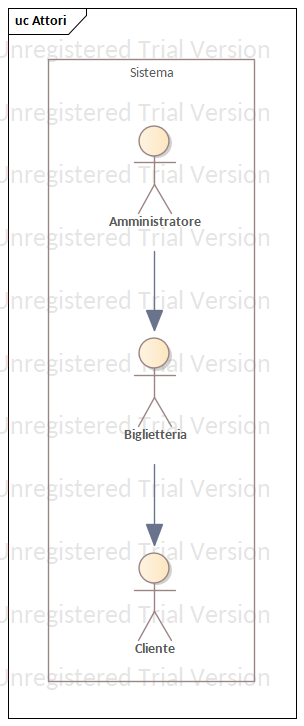
\includegraphics{imgs/use_case/attori}

        \subsection{Cliente}
            \subsubsection{Diagramma}
                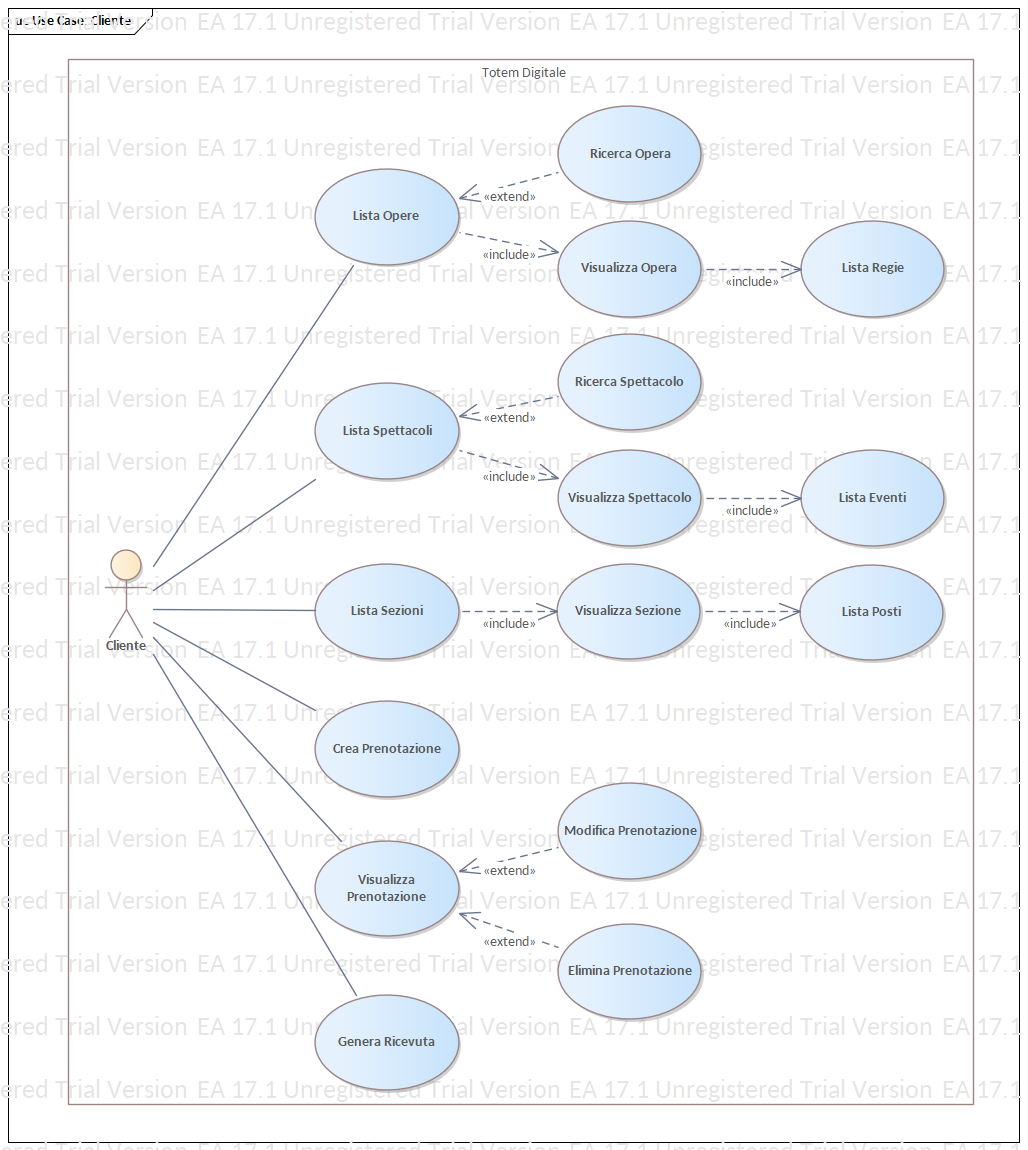
\includegraphics[width=\textwidth]{imgs/use_case/cliente}

            \subsubsection{Descrizioni}
                % UC: Lista Opere
                \begin{table}[H]
                    \begin{tabular}{|p{\linewidth}|}
                        \hline
                        \cellcolor{gray!100}
                        \color{white}
                        \centerline{\textbf{Caso d'uso:} Lista Opere} \\
                        \hline
                        \textbf{ID:} 1 \\
                        \hline
                        \cellcolor{gray!20}
                        \textbf{Breve descrizione:} \\
                        \cellcolor{gray!20}
                        L'utente ottiene la lista di opere memorizzate nel sistema. \\
                        \hline
                        \textbf{Attori primari:} \\
                        \begin{minipage}{\linewidth}
                            Cliente \\
                            Biglietteria \\
                            Amministratore
                        \end{minipage}
                        \vspace{0pt} \\  % Utilizzo \vspace{} per regolare lo spazio tra le sezioni delle tabelle.
                        \hline
                        \textbf{Attori secondari:} \\
                        Nessuno. \\
                        \hline
                        \cellcolor{gray!20}
                        \textbf{Precondizioni:} \\
                        \cellcolor{gray!20}
                        \begin{minipage}{\linewidth}
                            \begin{enumerate}
                                \item L'utente è posizionato nella sezione informazioni.
                            \end{enumerate}
                        \end{minipage} \\
                        \hline
                        \textbf{Sequenza degli eventi principale:}
                        \begin{enumerate}
                            \item Il caso d'uso inizia quando l'utente entra nella sezione informazioni.
                            \item \textbf{If} nel sistema è memorizzata almeno un'opera
                            \begin{enumerate}
                                \item \textbf{For} ogni opera nel sistema
                                \begin{enumerate}
                                    \item[] \textbf{punto di estensione:} filtro ricerca
                                    \item \textbf{include}(Visualizza Opera)
                                \end{enumerate}
                            \end{enumerate}
                            \item \textbf{Else}
                            \begin{enumerate}
                                \item Il sistema informa l'utente che non vi sono opere memorizzate.
                            \end{enumerate}
                        \end{enumerate} \\
                        \hline
                        \cellcolor{gray!20}
                        \textbf{Postcondizioni:} \\
                        \cellcolor{gray!20}
                        \begin{minipage}{\linewidth}
                            \begin{enumerate}
                                \item Viene visualizzata a schermo la lista delle opere memorizzate.
                            \end{enumerate}
                        \end{minipage} \\
                        \hline
                        \textbf{Sequenza degli eventi alternativa:} \\
                        Nessuna. \\
                        \hline
                    \end{tabular}
                \end{table}

                % UC EXT: Ricerca Opera
                \begin{table}[H]
                    \begin{tabular}{|p{\linewidth}|}
                        \hline
                        \cellcolor{gray!100}
                        \color{white}
                        \centerline{\textbf{Caso d'uso:} Ricerca Opera} \\
                        \hline
                        \textbf{ID:} 2 \\
                        \hline
                        \cellcolor{gray!20}
                        \textbf{Breve descrizione:} \\
                        \cellcolor{gray!20}
                        \textbf{Segmento 1:} L'utente filtra la lista di opere tramite parola chiave ricercata nel nome. \\
                        \hline
                        \textbf{Attori primari:} \\
                        \begin{minipage}{\linewidth}
                            Cliente \\
                            Biglietteria \\
                            Amministratore
                        \end{minipage}
                        \vspace{0pt} \\  % Utilizzo \vspace{} per regolare lo spazio tra le sezioni delle tabelle.
                        \hline
                        \textbf{Attori secondari:} \\
                        Nessuno. \\
                        \hline
                        \cellcolor{gray!20}
                        \textbf{Precondizioni:} \\
                        \cellcolor{gray!20}
                        \begin{minipage}{\linewidth}
                            \begin{enumerate}
                                \item L'utente ha inserito una chiave di ricerca.
                                \item L'utente ha premuto il pulsante di ricerca.
                            \end{enumerate}
                        \end{minipage} \\
                        \hline
                        \textbf{Sequenza degli eventi principale:}
                        \begin{enumerate}
                            \item Le opere che non contengono la parola chiave vengono eliminate dalla lista risultante.
                        \end{enumerate} \\
                        \hline
                        \cellcolor{gray!20}
                        \textbf{Postcondizioni:} \\
                        \cellcolor{gray!20}
                        \begin{minipage}{\linewidth}
                            \begin{enumerate}
                                \item La lista risultante è filtrata.
                            \end{enumerate}
                        \end{minipage} \\
                        \hline
                        \textbf{Sequenza degli eventi alternativa:} \\
                        Nessuna. \\
                        \hline
                    \end{tabular}
                \end{table}

                % UC: Visualizza Opera
                \begin{table}[H]
                    \begin{tabular}{|p{\linewidth}|}
                        \hline
                        \cellcolor{gray!100}
                        \color{white}
                        \centerline{\textbf{Caso d'uso:} Visualizza Opera} \\
                        \hline
                        \textbf{ID:} 3 \\
                        \hline
                        \cellcolor{gray!20}
                        \textbf{Breve descrizione:} \\
                        \cellcolor{gray!20}
                        L'utente ottiene le informazioni anagrafiche riguardo una singola opera. \\
                        \hline
                        \textbf{Attori primari:} \\
                        \begin{minipage}{\linewidth}
                            Cliente \\
                            Biglietteria \\
                            Amministratore
                        \end{minipage}
                        \vspace{0pt} \\  % Utilizzo \vspace{} per regolare lo spazio tra le sezioni delle tabelle.
                        \hline
                        \textbf{Attori secondari:} \\
                        Nessuno. \\
                        \hline
                        \cellcolor{gray!20}
                        \textbf{Precondizioni:} \\
                        \cellcolor{gray!20}
                        \begin{minipage}{\linewidth}
                            \begin{enumerate}
                                \item L'utente è posizionato nella sezione informazioni.
                            \end{enumerate}
                        \end{minipage} \\
                        \hline
                        \textbf{Sequenza degli eventi principale:}
                        \begin{enumerate}
                            \item Il caso d'uso inizia quando l'utente richiede le informazioni di un'opera.
                            \item Il sistema cerca le informazioni anagrafiche nella memoria in base all'identificativo dell'opera.
                            \item Il sistema mostra le informazioni a schermo.
                            \item \textbf{include}(Lista Regie)
                            \item[] \textbf{punto di estensione:} modifica
                        \end{enumerate} \\
                        \hline
                        \cellcolor{gray!20}
                        \textbf{Postcondizioni:} \\
                        \cellcolor{gray!20}
                        \begin{minipage}{\linewidth}
                            \begin{enumerate}
                                \item Sono visualizzate a schermo le informazioni anagrafiche dell'opera.
                            \end{enumerate}
                        \end{minipage} \\
                        \hline
                        \textbf{Sequenza degli eventi alternativa:} \\
                        Nessuna. \\
                        \hline
                    \end{tabular}
                \end{table}

                % UC: Lista Regie
                \begin{table}[H]
                    \begin{tabular}{|p{\linewidth}|}
                        \hline
                        \cellcolor{gray!100}
                        \color{white}
                        \centerline{\textbf{Caso d'uso:} Lista Regie} \\
                        \hline
                        \textbf{ID:} 4 \\
                        \hline
                        \cellcolor{gray!20}
                        \textbf{Breve descrizione:} \\
                        \cellcolor{gray!20}
                        L'utente ottiene la lista di regie relative all'opera che sta visualizzando. \\
                        \hline
                        \textbf{Attori primari:} \\
                        \begin{minipage}{\linewidth}
                            Cliente \\
                            Biglietteria \\
                            Amministratore
                        \end{minipage}
                        \vspace{0pt} \\  % Utilizzo \vspace{} per regolare lo spazio tra le sezioni delle tabelle.
                        \hline
                        \textbf{Attori secondari:} \\
                        Nessuno. \\
                        \hline
                        \cellcolor{gray!20}
                        \textbf{Precondizioni:} \\
                        \cellcolor{gray!20}
                        \begin{minipage}{\linewidth}
                            \begin{enumerate}
                                \item L'utente sta visualizzando una singola opera.
                            \end{enumerate}
                        \end{minipage} \\
                        \hline
                        \textbf{Sequenza degli eventi principale:}
                        \begin{enumerate}
                            \item Il caso d'uso inizia quando l'utente visualizza una singola opera.
                            \item \textbf{If} per l'opera è memorizzata almeno una regia
                            \begin{enumerate}
                                \item \textbf{For} ogni regia dell'opera
                                \begin{enumerate}
                                    \item Il sistema mostra le informazioni della regia a schermo.
                                \end{enumerate}
                            \end{enumerate}
                            \item \textbf{Else}
                            \begin{enumerate}
                                \item Il sistema informa l'utente che non vi sono regie memorizzate.
                            \end{enumerate}
                        \end{enumerate} \\
                        \hline
                        \cellcolor{gray!20}
                        \textbf{Postcondizioni:} \\
                        \cellcolor{gray!20}
                        \begin{minipage}{\linewidth}
                            \begin{enumerate}
                                \item E' visualizzata a schermo la lista delle regie associate all'opera.
                            \end{enumerate}
                        \end{minipage} \\
                        \hline
                        \textbf{Sequenza degli eventi alternativa:} \\
                        Nessuna. \\
                        \hline
                    \end{tabular}
                \end{table}

                % Caso d'uso: CreaPrenotazione
                \begin{table}[H]
                    \begin{tabular}{|p{\linewidth}|}
                        \hline
                        \cellcolor{gray!100}
                        \color{white}
                        \centerline{\textbf{Caso d'uso:} CreaPrenotazione} \\
                        \hline
                        \textbf{ID:} -POR DEFINIR- \\
                        \hline
                        \cellcolor{gray!20}
                        \textbf{Breve descrizione:} 
                            
                        Questo caso d'uso consente all'utente prenotare posti di eventi svolti nel teatro. \\
                        \hline
                        \textbf{Attori primari:} \\
                        \begin{minipage}{\linewidth}
                            \begin{enumerate}
                                \item Amministratore;
                                \item Biglietteria;
                                \item Cliente.
                            \end{enumerate}
                        \end{minipage}
                        \vspace{0pt} \\  % Utilizzo \vspace{} per regolare lo spazio tra le sezioni delle tabelle.
                        \hline
                        \textbf{Attori secondari:}
                        
                        Nessuno. \\
                        \hline
                        \cellcolor{gray!20}
                        \textbf{Precondizioni:} \\
                        \cellcolor{gray!20}
                        \begin{minipage}{\linewidth}
                            \begin{enumerate}
                                \item L'utente visualizza l'elenco degli eventi. % NON NE SONO CONVINTO.
                            \end{enumerate}
                        \end{minipage} \\
                        \hline
                        \textbf{Sequenza degli eventi principale:}
                        \begin{enumerate}
                            \item Il caso d'uso inizia quando l'utente preme "Creare prenotazione";
                            \item Il sistema mostra una interfaccia per inserire i dati relativi alla prenotazione;
                            \item L'utente inserisce i dati relativi alla prenotazione; 
                            \item L'utente preme "Salva";
                            \item \textit{If} i dati inseriti sono validi
                            \begin{enumerate}
                                \item Il sistema salva i dati;
                                \item \textit{If} l'utente è Cliente
                                \begin{enumerate}
                                    \item L'utente è inviato alla categoria "Prenotazioni";
                                \end{enumerate}
                                \item Il caso d'uso finisce.
                            \end{enumerate}
                            \item \textit{Else}
                            \begin{enumerate}
                                \item Il sistema mostra un messaggio d'errore;
                                \item L'utente torna al passo 3;
                            \end{enumerate}
                        \end{enumerate} \\
                        \hline
                        \cellcolor{gray!20}
                        \textbf{Postcondizioni:} \\
                        \cellcolor{gray!20}
                        \begin{minipage}{\linewidth}
                            \begin{enumerate}
                                \item L'utente crea una prenotazione; % Anche se ridondante, è meglio di mettere "Nessuna.".
                                \item Se l'utente è Cliente, è inviato alla categoria "Prenotazioni".
                            \end{enumerate}
                        \end{minipage}
                        \vspace{-5pt} \\
                        \hline
                        \textbf{Sequenza degli eventi alternativa:}
                        
                        Nessuna. \\
                        \hline
                    \end{tabular}
                \end{table}

                % Caso d'uso: VisualizzaPrenotazione
                \begin{table}[H]
                    \begin{tabular}{|p{\linewidth}|}
                        \hline
                        \cellcolor{gray!100}
                        \color{white}
                        \centerline{\textbf{Caso d'uso:} VisualizzaPrenotazione} \\
                        \hline
                        \textbf{ID:} -POR DEFINIR- \\
                        \hline
                        \cellcolor{gray!20}
                        \textbf{Breve descrizione:}

                        Questo caso d'uso consente di visualizzare una particolare prenotazione in modo più dettagliato. \\
                        \hline
                        \textbf{Attori primari:} \\
                        \begin{minipage}{\linewidth}
                            \begin{enumerate}
                                \item Amministratore;
                                \item Biglietteria;
                                \item Cliente.
                            \end{enumerate}
                        \end{minipage}
                        \vspace{0pt} \\
                        \hline
                        \textbf{Attori secondari:}

                        Nessuno. \\
                        \hline
                        \cellcolor{gray!20}
                        \textbf{Precondizioni:} \\
                        \cellcolor{gray!20}
                        \begin{minipage}{\linewidth}
                            \begin{enumerate}
                                \item L'utente si trova nella categoria "Prenotazioni";
                                \item L'elenco delle prenotazioni, sia esso filtrato o meno, non è vuoto.
                            \end{enumerate}
                        \end{minipage}
                        \vspace{-5pt} \\
                        \hline
                        \textbf{Sequenza degli eventi principale:}
                        \begin{enumerate}
                            \item \textit{If} l'utente è Cliente
                            \begin{enumerate}
                                \item Il sistema agisce sulla prenotazione creata dal Cliente;
                            \end{enumerate}
                            \item Il sistema mostra gli attributo relativi alla prenotazione; % Dovrei mettere più dettagli.
                            \item Il sistema mostra tre pulsanti vincolati alla prenotazione: "Modifica", "Elimina" e "Segnare";
                            \item \textit{If} l'utente è Cliente
                            \begin{enumerate}
                                \item Il sistema mostra il pulsante "Genera ricevuta";
                                \item[] \hspace*{-\tabcolsep} \textit{extension point}: modificaPrenotazione
                            \end{enumerate}
                        \end{enumerate} \\
                        \hline
                        \cellcolor{gray!20}
                        \textbf{Postcondizioni:} \\
                        \cellcolor{gray!20}
                        \begin{minipage}{\linewidth}
                            \begin{enumerate}
                                \item L'utente visualizza una prenotazione;
                                \item Il sistema mostra tre pulsanti relativi alla prenotazione;
                                \item Se l'utente è Cliente, i tre pulsanti sono funzionali.
                            \end{enumerate}
                        \end{minipage}
                        \vspace{0pt} \\
                        \hline
                        \textbf{Sequenza degli eventi alternativa:}

                        Nessuna. \\
                        \hline
                    \end{tabular}
                \end{table}

                % Caso d'uso dell'estensione: ModificaPrenotazione
                \begin{table}[H]
                    \begin{tabular}{|p{\linewidth}|}
                        \hline
                        \cellcolor{gray!100}
                        \color{white}
                        \centerline{\textbf{Caso d'uso dell'estensione:} ModificaPrenotazione} \\
                        \hline
                        \textbf{ID:} -POR DEFINIR- \\
                        \hline
                        \cellcolor{gray!20}
                        \textbf{Breve descrizione:}
                        
                        Segmento 1: L'utente modifica una prenotazione esistente all'interno dell'elenco delle prenotazioni. \\
                        \hline
                        \textbf{Attori principali:} \\
                        \begin{minipage}{\linewidth}
                            \begin{enumerate}
                                \item Amministratore;
                                \item Biglietteria;
                                \item Cliente. % EL CLIENTE PUEDE MODIFICAR LA PRENOTAZIONE
                            \end{enumerate}
                        \end{minipage}
                        \vspace{0pt} \\
                        \hline
                        \textbf{Attori secondari:}
                        
                        Nessuno. \\
                        \hline
                        \cellcolor{gray!20}
                        \textbf{Precondizioni del segmento 1:} \\
                        \cellcolor{gray!20}
                        \begin{minipage}{\linewidth}
                            \begin{enumerate}
                                \item L'utente visualizza l'elenco delle prenotazioni;
                                \item L'utente preme "Modifica".
                            \end{enumerate}
                        \end{minipage}
                        \vspace{-5pt} \\
                        \hline
                        \textbf{Sequenza degli eventi del segmento 1:}
                        \begin{enumerate}
                            \item Il sistema mostra la interfaccia di creazione di prenotazione, ma con un dati saltavi della prenotazione già creata selezionati; % Da confirmare coi ragazzi.
                            \item L'utente modifica i dati relativi alla prenotazione;
                            \item L'utente preme "Salva";
                            \item \textit{If} i dati sono validi
                            \begin{enumerate}
                                \item Il sistema salva i dati;
                                \item Il caso d'uso finisce.
                            \end{enumerate}
                            \item \textit{Else}
                            \begin{enumerate}
                                \item Il sistema mostra un messaggio di errore;
                                \item L'utente torna al passo 2;
                            \end{enumerate}
                        \end{enumerate} \\
                        \hline
                        \cellcolor{gray!20}
                        \textbf{Postcondizioni del segmento 1:} \\
                        \cellcolor{gray!20}
                        \begin{minipage}{\linewidth}
                            \begin{enumerate}
                                \item L'utente effettua la modifica di una prenotazione.
                            \end{enumerate}
                        \end{minipage} \\
                        \hline
                    \end{tabular}
                \end{table}

                % Caso d'uso dell'estensione: EliminaPrenotazione
                \begin{table}[H]
                    \begin{tabular}{|p{\linewidth}|}
                        \hline
                        \cellcolor{gray!100}
                        \color{white}
                        \centerline{\textbf{Caso d'uso dell'estensione:} EliminaPrenotazione} \\
                        \hline
                        \textbf{ID:} -POR DEFINIR- \\
                        \hline
                        \cellcolor{gray!20}
                        \textbf{Breve descrizione:}
                        
                        Segmento 1: L'utente elimina una prenotazione esistente all'interno dell'elenco delle prenotazioni. \\
                        \hline
                        \textbf{Attori principali:} \\
                        \begin{minipage}{\linewidth}
                            \begin{enumerate}
                                \item Amministratore;
                                \item Biglietteria;
                                \item Cliente.
                            \end{enumerate}
                        \end{minipage}
                        \vspace{0pt} \\
                        \hline
                        \textbf{Attori secondari:}
                        
                        Nessuno. \\
                        \hline
                        \cellcolor{gray!20}
                        \textbf{Precondizioni del segmento 1:} \\
                        \cellcolor{gray!20}
                        \begin{minipage}{\linewidth}
                            \begin{enumerate}
                                \item L'utente visualizza l'elenco delle prenotazioni;
                                \item L'utente preme "Elimina".
                            \end{enumerate}
                        \end{minipage}
                        \vspace{-5pt} \\
                        \hline
                        \textbf{Sequenza degli eventi del segmento 1:}
                        \begin{enumerate}
                            \item Il sistema chiede conferma per eliminare la prenotazione;
                            \item \textit{If} l'utente preme "Conferma"
                            \begin{enumerate}
                                \item Il sistema effettua l'eliminazione della prenotazione;
                                \item Il sistema torna all'elenco delle prenotazioni;
                                \item Il sistema mostra un messaggio chiarendo che l'eliminazione è stata effettuata;
                                \item L'utente chiude la finestra del messaggio.
                            \end{enumerate}
                        \end{enumerate} \\
                        \hline
                        \cellcolor{gray!20}
                        \textbf{Postcondizioni del segmento 1:} \\
                        \cellcolor{gray!20}
                        \begin{minipage}{\linewidth}
                            \begin{enumerate}
                                \item L'utente effettua l'eliminazione di una prenotazione.
                            \end{enumerate}
                        \end{minipage} \\
                        \hline
                    \end{tabular}
                \end{table}

                %% ESTE CASO DE USO ES PARA EL CLIENTE Y VA VINCULADO A VisualizzaPrenotazione
                % Caso d'uso: GeneraRicevuta
                \begin{table}[H]
                    \begin{tabular}{|p{\linewidth}|}
                        \hline
                        \cellcolor{gray!100}
                        \color{white}
                        \centerline{\textbf{Caso d'uso:} GeneraRicevuta} \\
                        \hline
                        \textbf{ID:} -POR DEFINIR- \\
                        \hline
                        \cellcolor{gray!20}
                        \textbf{Breve descrizione:}

                        Questo caso d'uso consente generare la ricevuta di una prenotazione. \\
                        \hline
                        \textbf{Attori primari:} \\
                        \begin{minipage}{\linewidth}
                            \begin{enumerate}
                                \item Amministratore;
                                \item Biglietteria;
                                \item Cliente.
                            \end{enumerate}
                        \end{minipage}
                        \vspace{0pt} \\
                        \hline
                        \textbf{Attori secondari:}

                        Nessuno. \\
                        \hline
                        \cellcolor{gray!20}
                        \textbf{Precondizioni:} \\
                        \cellcolor{gray!20}
                        \begin{minipage}{\linewidth}
                            \begin{enumerate}
                                \item L'utente visualizza l'elenco delle prenotazioni. % Da confrontare col diagramma dei casi d'uso dei Clienti.
                            \end{enumerate}
                        \end{minipage} \\
                        \hline
                        \textbf{Sequenza degli eventi principale:}
                        \begin{enumerate}
                            \item Il caso d'uso comincia quando l'utente preme "Generare ricevuta";
                            \item Il sistema genera un documento con tutta l'informazione relativa all'acquisto dei biglietti prenotati;
                            \item Il sistema stampa la ricevuta.
                        \end{enumerate} \\
                        \hline
                        \cellcolor{gray!20}
                        \textbf{Postcondizioni:} \\
                        \cellcolor{gray!20}
                        \begin{minipage}{\linewidth}
                            \begin{enumerate}
                                \item La ricevuta è stata stampata.
                            \end{enumerate}
                        \end{minipage} \\
                        \hline
                        \textbf{Sequenza degli eventi alternativa:}
                        
                        Nessuna. \\
                        \hline
                    \end{tabular}
                \end{table}

                % Caso d'uso: CreaSpettacolo (._.=)

                % Caso d'uso: CreaOpera (=R)

        \subsection{Biglietteria}
            \subsubsection{Diagramma}
                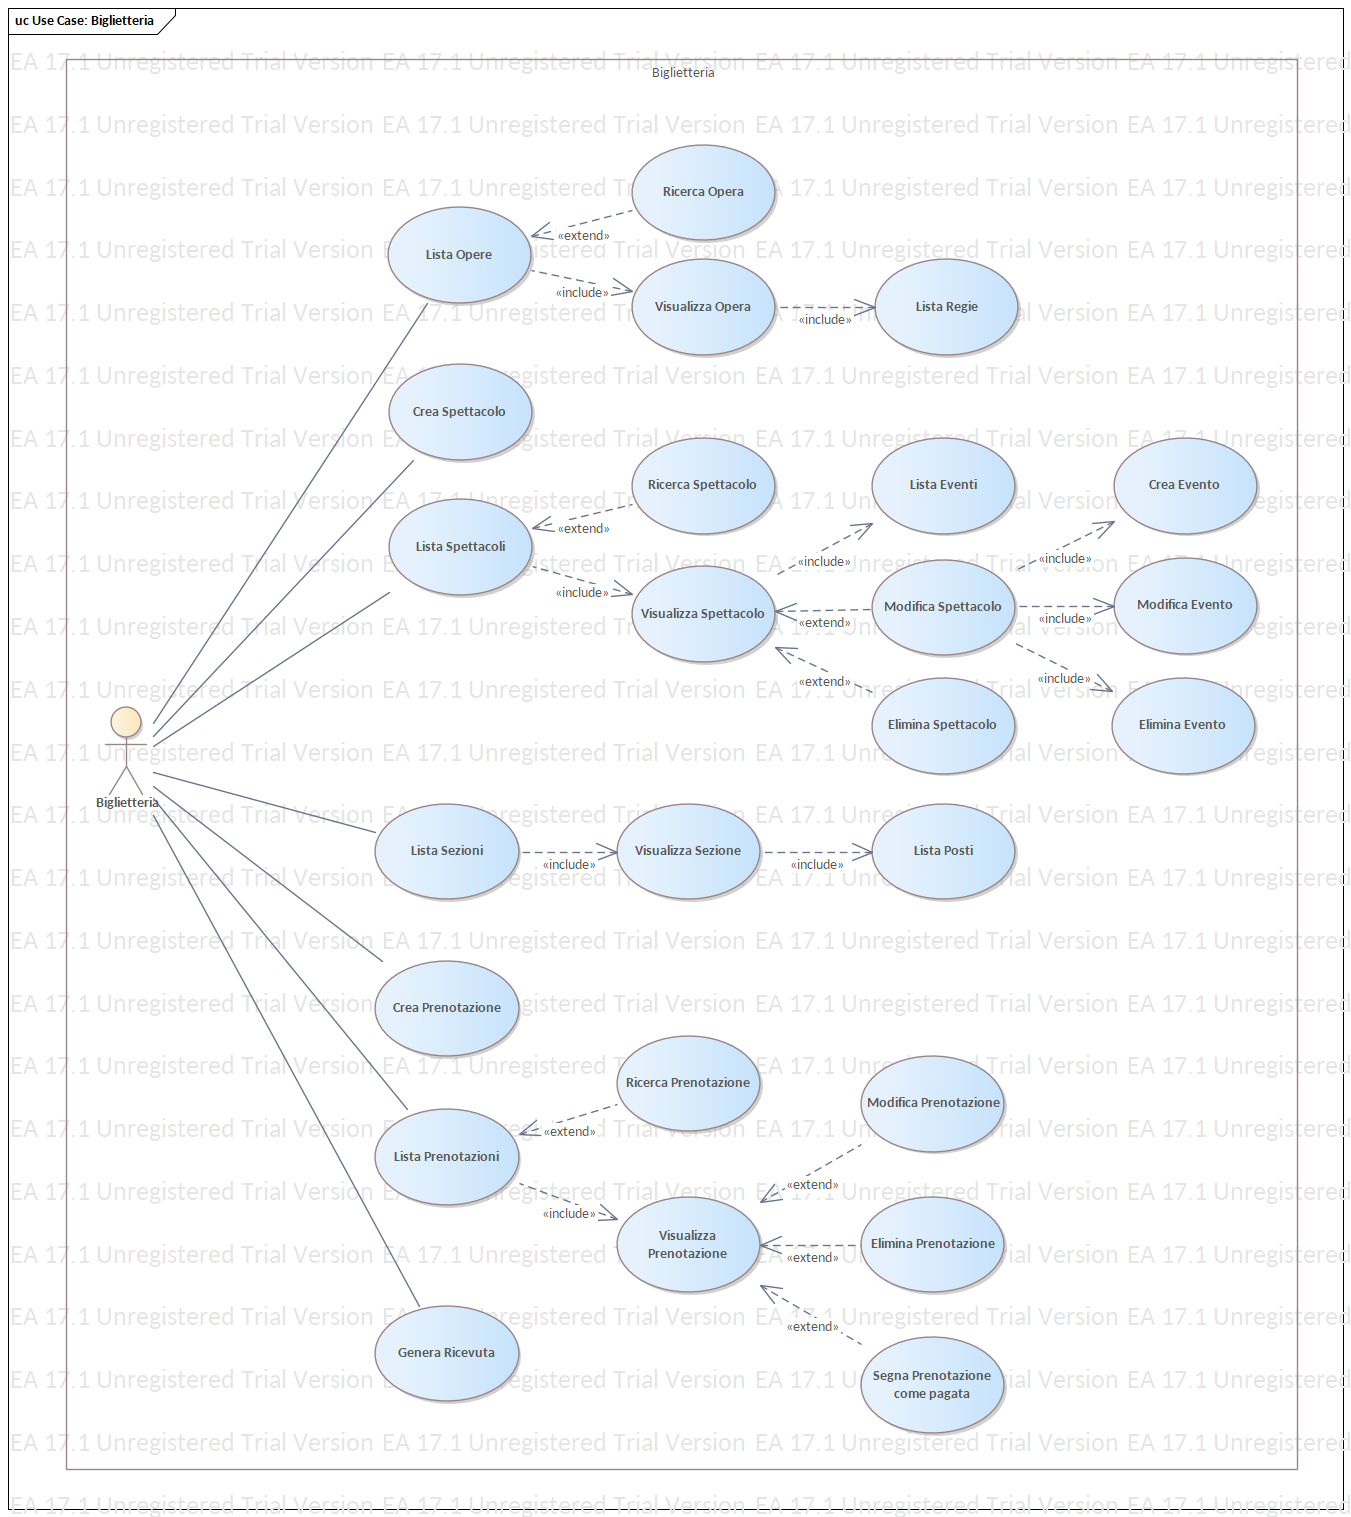
\includegraphics[width=\textwidth]{imgs/use_case/biglietteria}
            
            \subsubsection{Descrizioni}
                % Caso d'uso: ListaPrenotazione
                \begin{table}[H]
                    \begin{tabular}{|p{\linewidth}|}
                        \hline
                        \cellcolor{gray!100}
                        \color{white}
                        \centerline{\textbf{Caso d'uso:} ListaPrenotazione} \\
                        \hline
                        \textbf{ID:} -POR DEFINIR- \\
                        \hline
                        \cellcolor{gray!20}
                        \textbf{Breve descrizione:}
                        
                        Questo caso d'uso consente visualizzare l'elenco delle prenotazione salvate nel sistema. \\
                        \hline
                        \textbf{Attori primari:} \\
                        \begin{minipage}{\linewidth}
                            \begin{enumerate}
                                \item Amministratore;
                                \item Biglietteria.
                            \end{enumerate}
                        \end{minipage}
                        \vspace {-5pt} \\
                        \hline
                        \textbf{Attori secondari:}
                        
                        Nessuno. \\
                        \hline
                        \cellcolor{gray!20}
                        \textbf{Precondizioni:} \\
                        \cellcolor{gray!20}
                        \begin{minipage}{\linewidth}
                            \begin{enumerate}
                                \item L'utente è stato autenticato come amministratore o personale di biglietteria;
                                \item L'utente si trova nella categoria "Prenotazioni". % Utilizo "categoria" per non confonderla con "sezione".
                            \end{enumerate}
                        \end{minipage}
                        \vspace{0pt} \\
                        \hline
                        \textbf{Sequenza degli eventi principale:}
                        \begin{enumerate}
                            \item Questo caso d'uso inizia dopo che l'utente seleziona la categoria "Prenotazioni";
                            \item \textit{If} c'è almeno una prenotazione salvata nel sistema
                            \begin{enumerate}
                                \item \textit{For} ogni prenotazione salvate nel sistema
                                \begin{enumerate}
                                    \item \textit{include}(VisualizzaPrenotazione)
                                \end{enumerate}
                                \begin{itemize}
                                    \item[] \hspace*{-\tabcolsep*3} \textit{extension point}: filtrareElenco
                                \end{itemize}
                                \item \textit{For} ogni prenotazione nell'elenco
                                \begin{itemize}
                                    \item[] \textit{extension point}: modificaEvento
                                \end{itemize}
                            \end{enumerate}
                            \item \textit{Else}
                            \begin{enumerate}
                                \item Il sistema indica all'utente che l'elenco delle prenotazioni è vuoto.
                            \end{enumerate}
                        \end{enumerate} \\
                        \hline
                        \cellcolor{gray!20}
                        \textbf{Postcondizioni:} \\
                        \cellcolor{gray!20}
                        \begin{minipage}{\linewidth}
                            \begin{enumerate}
                                \item L'utente visualizza l'elenco delle prenotazioni salvati nel sistema.
                                \item L'utente ha l'opzione di agire sulle prenotazioni, modificandole, eliminandole o segnandole come pagate.
                            \end{enumerate}  
                        \end{minipage}
                        \vspace{0pt} \\
                        \hline
                        \textbf{Sequenza degli eventi alternativa:}
                        
                        Nessuna. \\
                        \hline
                    \end{tabular}
                \end{table}

                % Caso d'uso dell'estensione: RicercaPrenotazione
                \begin{table}[H]
                    \begin{tabular}{|p{\linewidth}|}
                        \hline
                        \cellcolor{gray!100}
                        \color{white}
                        \centerline{\textbf{Caso d'uso d'estensione:} RicercaPrenotazione} \\
                        \hline
                        \textbf{ID:} -POR DEFINIR- \\
                        \hline
                        \cellcolor{gray!20}
                        \textbf{Breve descrizione:}

                        Segmento 1: Questo caso d'uso consente di filtrare l'elenco delle prenotazioni attraverso una ricerca. \\
                        \hline
                        \textbf{Attori primari:} \\
                        \begin{minipage}{\linewidth}
                            \begin{enumerate}
                                \item Amministratore;
                                \item Biglietteria.
                            \end{enumerate}
                        \end{minipage}
                        \vspace{-5pt} \\
                        \hline
                        \textbf{Attori secondari:}

                        Nessuno. \\
                        \hline
                        \cellcolor{gray!20}
                        \textbf{Precondizioni del segmento 1:} \\
                        \cellcolor{gray!20}
                        \begin{minipage}{\linewidth}
                            \begin{enumerate}
                                \item L'utente visualizza l'elenco delle prenotazioni.
                            \end{enumerate}
                        \end{minipage} \\
                        \hline
                        \textbf{Sequenza degli eventi del segmento 1:}
                        \begin{enumerate}
                            \item L'utente inserisce i criteri di ricerca;
                            \item Il sistema ricerca, nell'elenco delle prenotazioni, delle prenotazioni coincidenti;
                            \item \textit{If} il sistema trova almeno una prenotazione coincidente
                            \begin{enumerate}
                                \item Il sistema mostra le prenotazioni coincidenti;
                            \end{enumerate}
                            \item \textit{Else}
                            \begin{enumerate}
                                \item Il sistema indica che non si ha trovato nessuna prenotazione coincidente.
                            \end{enumerate}
                        \end{enumerate} \\
                        \hline
                        \cellcolor{gray!20}
                        \textbf{Postcondizioni del segmento 1:} \\
                        \cellcolor{gray!20}
                        \begin{minipage}{\linewidth}
                            \begin{enumerate}
                                \item L'utente visualizza l'elenco filtrato.
                            \end{enumerate}
                        \end{minipage} \\
                        \hline
                    \end{tabular}
                \end{table}

                % Caso d'uso dell'estensione: SegnaPagaPrenotazione
                \begin{table}[H]
                    \begin{tabular}{|p{\linewidth}|}
                        \hline
                        \cellcolor{gray!100}
                        \color{white}
                        \centerline{\textbf{Caso d'uso dell'estensione:} SegnaPagaPrenotazione} \\
                        \hline
                        \textbf{ID:} -POR DEFINIR- \\
                        \hline
                        \cellcolor{gray!20}
                        \textbf{Breve descrizione:}
                        
                        Segmento 1: L'utente segna una prenotazione come \emph{pagata}. \\
                        \hline
                        \textbf{Attori principali:} \\
                        \begin{minipage}{\linewidth}
                            \begin{enumerate}
                                \item Amministratore;
                                \item Biglietteria.
                            \end{enumerate}
                        \end{minipage}
                        \vspace{-5pt} \\
                        \hline
                        \textbf{Attori secondari:}
                        
                        Nessuno. \\
                        \hline
                        \cellcolor{gray!20}
                        \textbf{Precondizioni del segmento 1:} \\
                        \cellcolor{gray!20}
                        \begin{minipage}{\linewidth}
                            \begin{enumerate}
                                \item L'utente visualizza l'elenco delle prenotazioni;
                                \item L'utente preme "Segnare".
                            \end{enumerate}
                        \end{minipage}
                        \vspace{-5pt} \\
                        \hline
                        \textbf{Sequenza degli eventi del segmento 1:}
                        \begin{enumerate}
                            \item Il sistema chiede conferma per segnare la prenotazione come \emph{pagata};
                            \item \textit{If} L'utente preme "Conferma"
                            \begin{enumerate}
                                \item Il sistema segna la prenotazione come \emph{pagata};
                                \item Il sistema torna al elenco delle prenotazioni;
                                \item Il sistema mostra un messaggio chiarendo che l'assegnamento è stato effettuato;
                                \item L'utente chiude la finestra del messaggio.
                            \end{enumerate}
                        \end{enumerate} \\
                        \hline
                        \cellcolor{gray!20}
                        \textbf{Postcondizioni del segmento 1:} \\
                        \cellcolor{gray!20}
                        \begin{minipage}{\linewidth}
                            \begin{enumerate}
                                \item L'utente effettua l'assegnamento di una prenotazione come \emph{pagata}.
                            \end{enumerate}
                        \end{minipage} \\
                        \hline
                    \end{tabular}
                \end{table}

        \subsection{Amministratore}
            \subsubsection{Diagramma}
                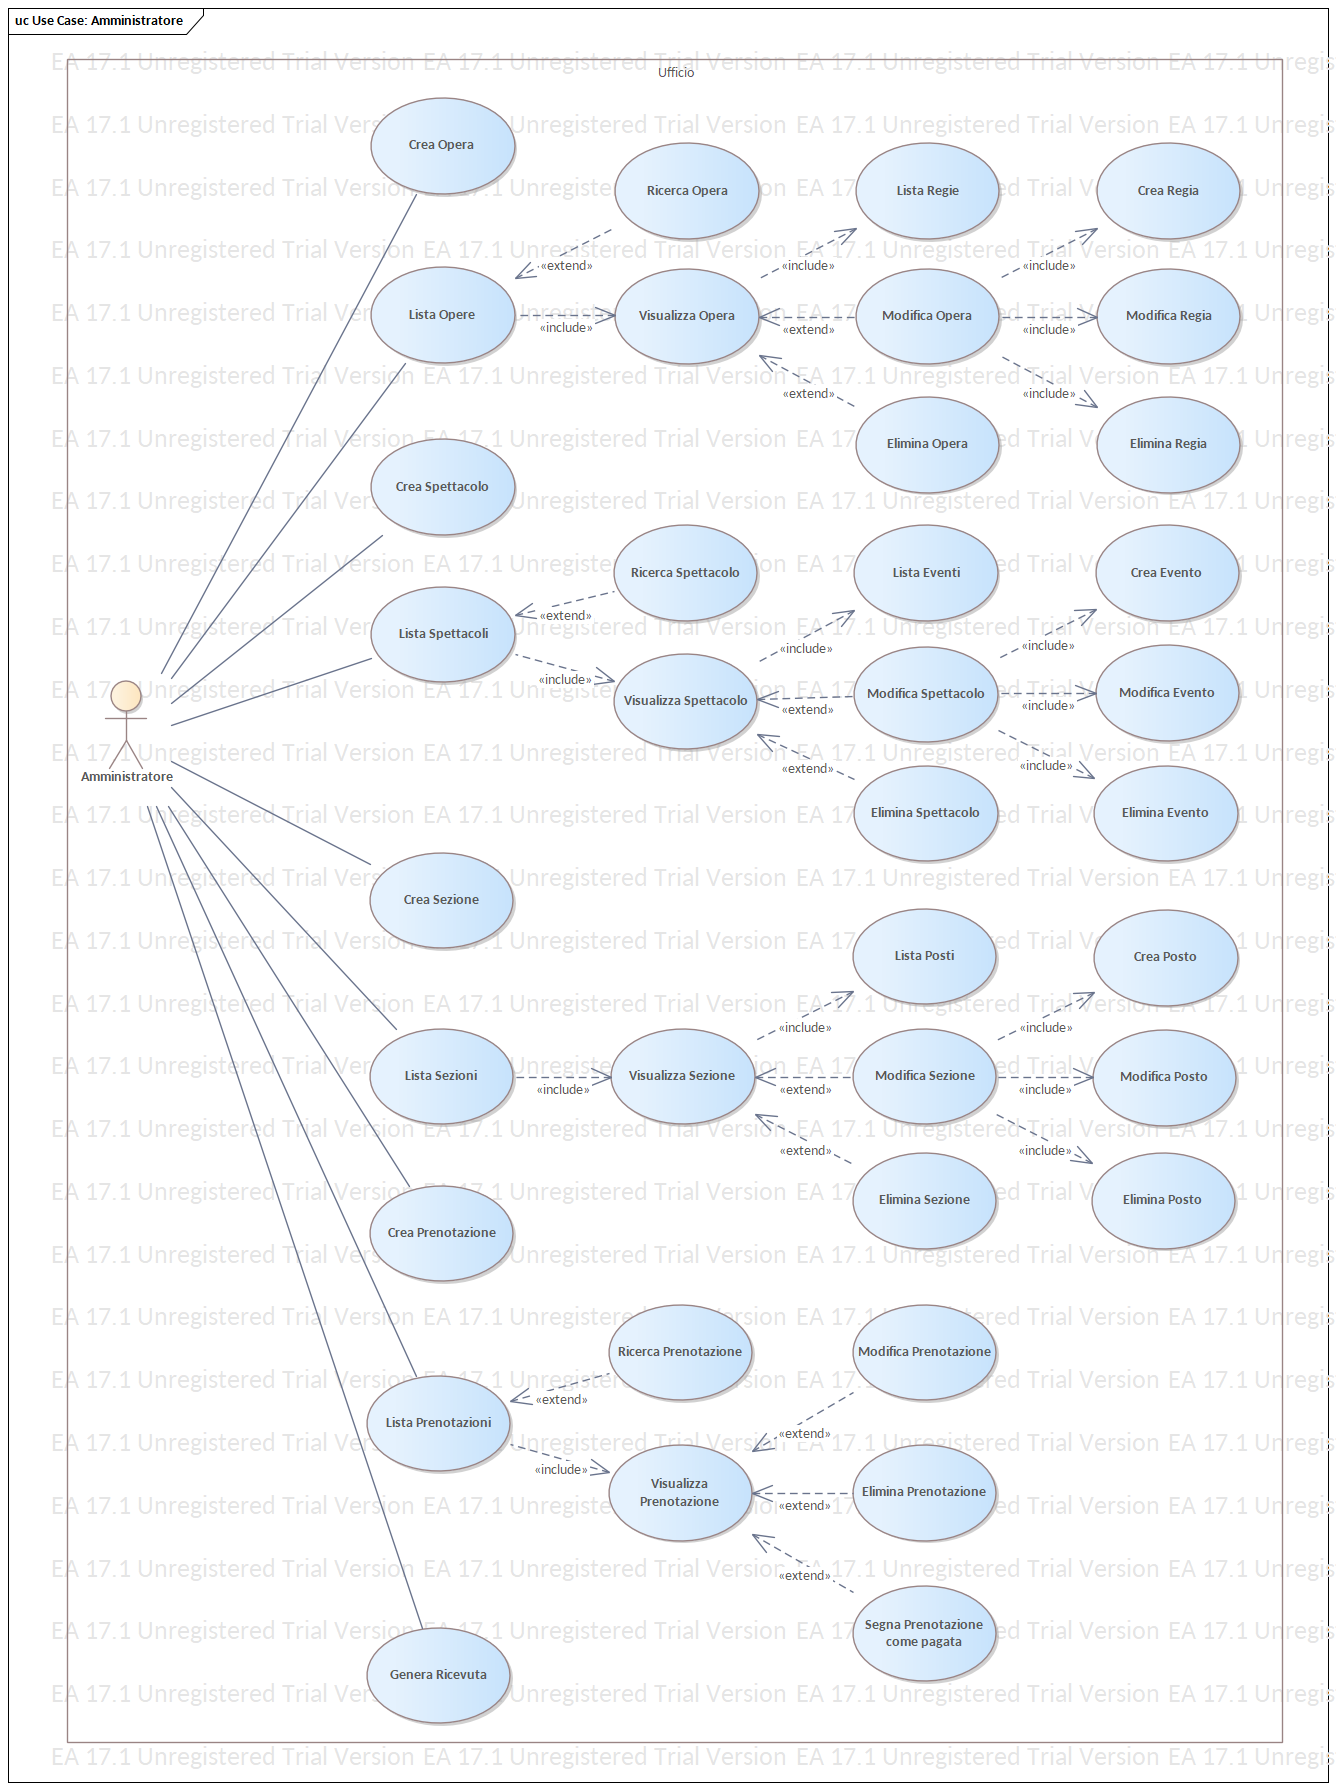
\includegraphics[width=\textwidth]{imgs/use_case/amministratore}

            \subsubsection{Descrizioni}

    \section{Matrice di mapping}
        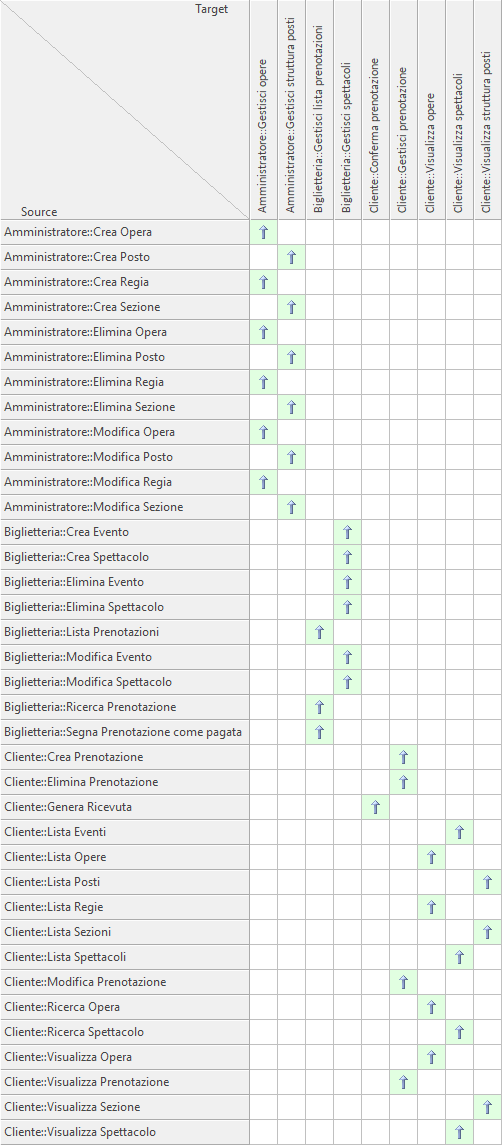
\includegraphics{imgs/matrice/matrice}

\end{document}
